\section{Material-UI}

Tento framework je implementací Material Designu od společnosti Google \cite{material-from-google}. Material-UI obsahuje spoustu připravených komponent, které jsou na míru šité pro tvorbu aplikací díky rozsáhle studii Googlu, která je pomocí zásad a instrukcí popsaná na vlastním webu\footnote{\url{https://material.io/guidelines/}}. Grafické rozhraní Aplikace je složeno z těchto komponent. Jedná se zejména o Appbar, Avatar, různé varianty pro Button, Card, Dialog, Drawer, Progress, formulářové prvky, Snackbar, Tabs a ikony\footnote{\url{https://material.io/icons/}}. Následují obrázkové ukázky:

\FloatBarrier

\begin{figure}[ht]
	\centering
	
\includegraphics[scale=0.5]{sections/ui/images/Appbar.png}
	\caption{Appbar}
	\label{fig:appbar}
\end{figure}

\begin{figure}[ht]
	\centering
	
\includegraphics[scale=0.5]{sections/ui/images/Avatar.png}
	\caption{Avatar}
	\label{fig:avatar}
\end{figure}

\begin{figure}[ht]
	\mbox{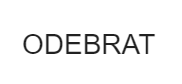
\includegraphics[scale=0.5]{sections/ui/images/Button-Flat.png}}   
	\hspace{12px}
	\mbox{
\includegraphics[scale=0.5]{sections/ui/images/Button-Raised.png}}
	\hspace{12px}
	\mbox{
\includegraphics[scale=0.5]{sections/ui/images/Button-Floating.png}}
	\hspace{12px}
	\mbox{
\includegraphics[scale=0.5]{sections/ui/images/Button-Icon.png}}
	\caption[Button]{Flat, Raised, Floating Action a Icon Button}
	\label{fig:buttons}
\end{figure}

\begin{figure}[ht]
	\centering
	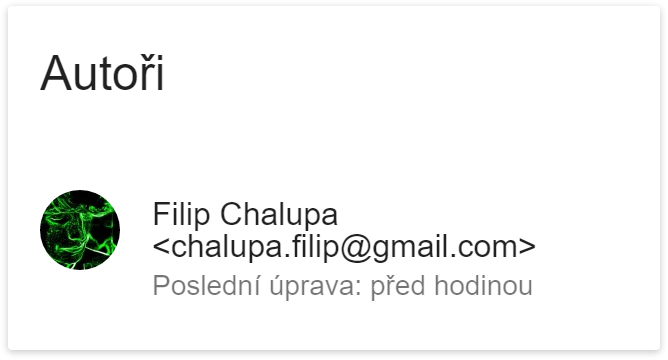
\includegraphics[scale=0.5]{sections/ui/images/Card.png}
	\caption[Card]{Card, rámeček sloužící k seskupení souvisejícího obsahu}
	\label{fig:card}
\end{figure}

\begin{figure}[ht]
	\centering
	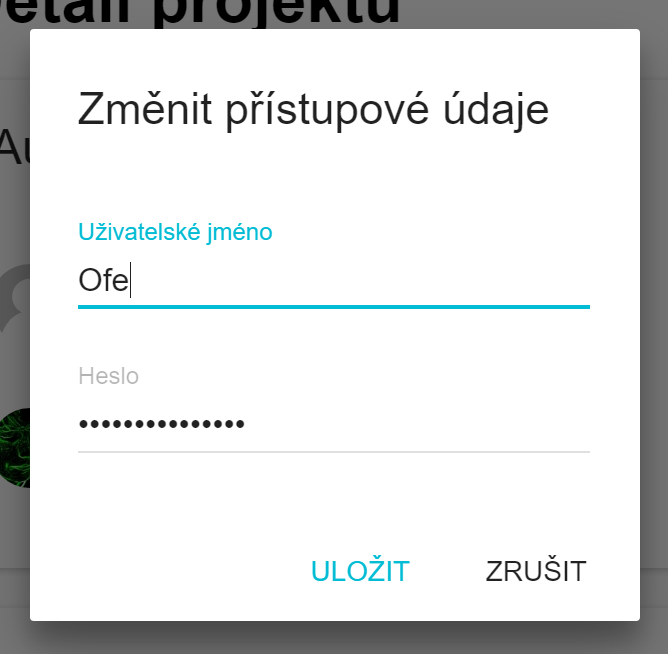
\includegraphics[scale=0.5]{sections/ui/images/Dialog.png}
	\caption[Dialog]{Dialog zobrazuje modální okna uvnitř aplikace}
	\label{fig:dialog}
\end{figure}

\begin{figure}[ht]
	\centering
	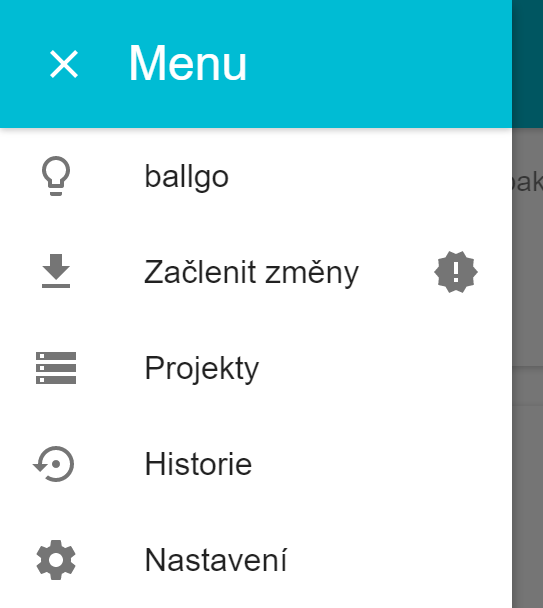
\includegraphics[scale=0.5]{sections/ui/images/Drawer.png}
	\caption[Drawer]{Drawer, boční vysouvací nabídka}
	\label{fig:drawer}
\end{figure}

\begin{figure}[ht]
	\centering
	
\includegraphics[scale=0.5]{sections/ui/images/Progress.png}
	\caption[Progress]{Znázornění právě probíhající akce. Například načítání historie projektu\footnote{Animované ukázky: \url{http://www.material-ui.com/\#/components/circular-progress}}}
	\label{fig:progress}
\end{figure}

\begin{figure}[ht]
	\mbox{
\includegraphics[scale=0.5]{sections/ui/images/TextField.png}}   
	\hspace{12px}
	\mbox{
\includegraphics[scale=0.5]{sections/ui/images/Checkbox.png}}
	\caption[TextField a Checkbox]{Text Field pro uživatelův textový vstup a Checkbox pro označování souborů}
	\label{fig:form}
\end{figure}

\begin{figure}[ht]
	\centering
	
\includegraphics[scale=0.5]{sections/ui/images/Tabs.png}
	\caption[Tabs]{Tabs pro skrytí osahu při přidávání projektu}
	\label{fig:tabs}
\end{figure}

\begin{figure}[ht]
	\centering
	
\includegraphics[scale=0.5]{sections/ui/images/Snackbar.png}
	\caption[Snackbar]{Snackbar, informační lišta ve spodní části okna o právě proběhlé akci}
	\label{fig:snackbar}
\end{figure}

\FloatBarrier
